\chapter{Training Every Model to 100 \% Training Accuracy}\label{ch:7}

The models of Chapters~\ref{ch:4}--\ref{ch:6} were stopped early on purpose: inner-validation early stopping, weight decay, dropout, shrinkage and augmentation keep their training accuracy at about 0.52--0.85 (Table~\ref{tab:3.3}). This chapter answers the question of what happens when that brake is removed. Every model that could be retrained here was trained again, with as many epochs or iterations as it needed, until its training accuracy reached (nearly) 100 \%, and was then measured on the same held-out data as before. The rules were written down and committed before any run (\texttt{research\_experiments/train100/AMENDMENT\_TRAIN100.md}, branch \texttt{research/train100}), and every number below is reported as it came out.

\section{Method}\label{sec:7.1}

Inputs, labels (the original four classes), network architectures, folds and decision rules were kept exactly as in the original runs; only the brakes on fitting were removed (Table~\ref{tab:7.1}). Models evaluated in development cross-validation use the same patient-grouped 5-fold split repeated three times, and the networks of the original project use its fixed training/validation split. Training accuracy is measured on all training ECGs of the fold in evaluation mode, without dropout or augmentation. The locked test set was not used, and no EchoNext data were used (Table~\ref{tab:7.7}).

\begin{table}[htbp]
\caption{What changed in TRAIN100. Inputs, labels, architectures, folds and decision rules are the original ones; only the brakes on fitting were removed, and every model was trained for as many epochs or iterations as it needed.}\label{tab:7.1}
\small
\begin{tabular}{>{\raggedright\arraybackslash\hspace{0pt}}p{\dimexpr 0.300\linewidth-2\tabcolsep\relax}>{\raggedright\arraybackslash\hspace{0pt}}p{\dimexpr 0.340\linewidth-2\tabcolsep\relax}>{\raggedright\arraybackslash\hspace{0pt}}p{\dimexpr 0.360\linewidth-2\tabcolsep\relax}}
\toprule
\textbf{Model family} & \textbf{Original training} & \textbf{TRAIN100 training} \\
\midrule
MLP heads and fusion networks & AdamW, weight decay chosen on inner validation, early stopping (patience 25) & weight decay 0, no early stopping, until 100 \% training accuracy (cap 3,000 epochs) \\
Linear and logistic models & L2 / C chosen on inner validation & L2 $10^{-6}$ or C = 10,000 \\
Gradient boosting & early stopping, shrinkage, L2 1, leaves chosen on inner validation & 2,000 trees, min\_child\_samples 1, L2 0, no early stopping \\
Image CNNs, 1-D SE-ResNet, ECGFounder fine-tuning & augmentation, label smoothing, EMA, weight decay 0.05, cosine schedule, early stopping & none of these; constant learning rate after warm-up, until training accuracy $\ge$ 99.5 \% (cap 100 / 150 / 60 epochs) \\
Ensembles, stacks, decision rules & weights, thresholds and prior rules chosen on inner out-of-fold predictions & same rules, same nesting, built from the TRAIN100 members; meta-learners C = 10,000 \\
\bottomrule
\end{tabular}
\end{table}


\section{Development cross-validation models}\label{sec:7.2}

Table~\ref{tab:7.2} and Figure~\ref{fig:7.1} compare the twelve main models. Every flexible model now fits its training data perfectly (1.000; C3 0.995), yet none becomes clearly better on held-out patients. The ensembles lose 2.6--3.8 points: IMG-C3 falls from 0.558 to 0.532, C3 from 0.561 to 0.533 and C1 from 0.547 to 0.517. The single networks lose 0.6--3.9 points. LightGBM is the only model that gains (0.524 to 0.548), inside its confidence interval. The image-only triage model keeps its accuracy on the patients it answers (0.696 against 0.694), but it now answers 48 \% of them instead of 56 \%, so it is slightly less useful. The three logistic regressions cannot reach 1.000 even with almost no regularisation (0.53--0.72): a model with straight-line class boundaries on a few dozen header or feature values cannot separate every training ECG, so this is a limit of the model type rather than of the training.

\begin{table}[htbp]
\caption{Development cross-validation (5 folds $\times$ 3 repeats, 837 ECGs): every model trained to (nearly) 100 \% training accuracy (TRAIN100; training and held-out columns) against the original early-stopped model. Held-out 95 \% CI corrected for repeated CV; change = TRAIN100 minus original, in percentage points.}\label{tab:7.2}
\small
\begin{tabular}{>{\raggedright\arraybackslash\hspace{0pt}}p{\dimexpr 0.270\linewidth-2\tabcolsep\relax}>{\raggedright\arraybackslash\hspace{0pt}}p{\dimexpr 0.155\linewidth-2\tabcolsep\relax}>{\raggedright\arraybackslash\hspace{0pt}}p{\dimexpr 0.270\linewidth-2\tabcolsep\relax}>{\raggedright\arraybackslash\hspace{0pt}}p{\dimexpr 0.160\linewidth-2\tabcolsep\relax}>{\raggedright\arraybackslash\hspace{0pt}}p{\dimexpr 0.145\linewidth-2\tabcolsep\relax}}
\toprule
\textbf{Model} & \textbf{Training accuracy} & \textbf{Held-out accuracy [95 \% CI]} & \textbf{Original held-out} & \textbf{Change (points)} \\
\midrule
HDR-LR & 0.529 & 0.483 [0.432, 0.535] & 0.489 & -0.6 \\
HDRCLIN-LR & 0.589 & 0.486 [0.436, 0.536] & 0.501 & -1.5 \\
CLIN-LR & 0.720 & 0.442 [0.390, 0.493] & 0.509 & -6.7 \\
LGBM-FEAT & 1.000 & 0.548 [0.512, 0.583] & 0.524 & +2.4 \\
ECGF-linear & 1.000 & 0.491 [0.451, 0.532] & 0.530 & -3.9 \\
ECGF-MLP & 1.000 & 0.536 [0.506, 0.565] & 0.542 & -0.6 \\
FUSION-MLP & 1.000 & 0.538 [0.499, 0.578] & 0.544 & -0.6 \\
C1 & 1.000 & 0.517 [0.477, 0.558] & 0.547 & -3.0 \\
C3 & 0.995 & 0.533 [0.496, 0.569] & 0.561 & -2.8 \\
IMG-vote & 1.000 & 0.503 [0.463, 0.544] & 0.541 & -3.8 \\
IMG-C3 & 1.000 & 0.532 [0.492, 0.572] & 0.558 & -2.6 \\
Image-only triage (AGT-img) & 1.000 (58 \% ans.) & 0.696 [0.630, 0.762] (48 \% ans.) & 0.694 (56 \% ans.) & +0.2 \\
\bottomrule
\end{tabular}
\end{table}


\begin{figure}[htbp]
\centering
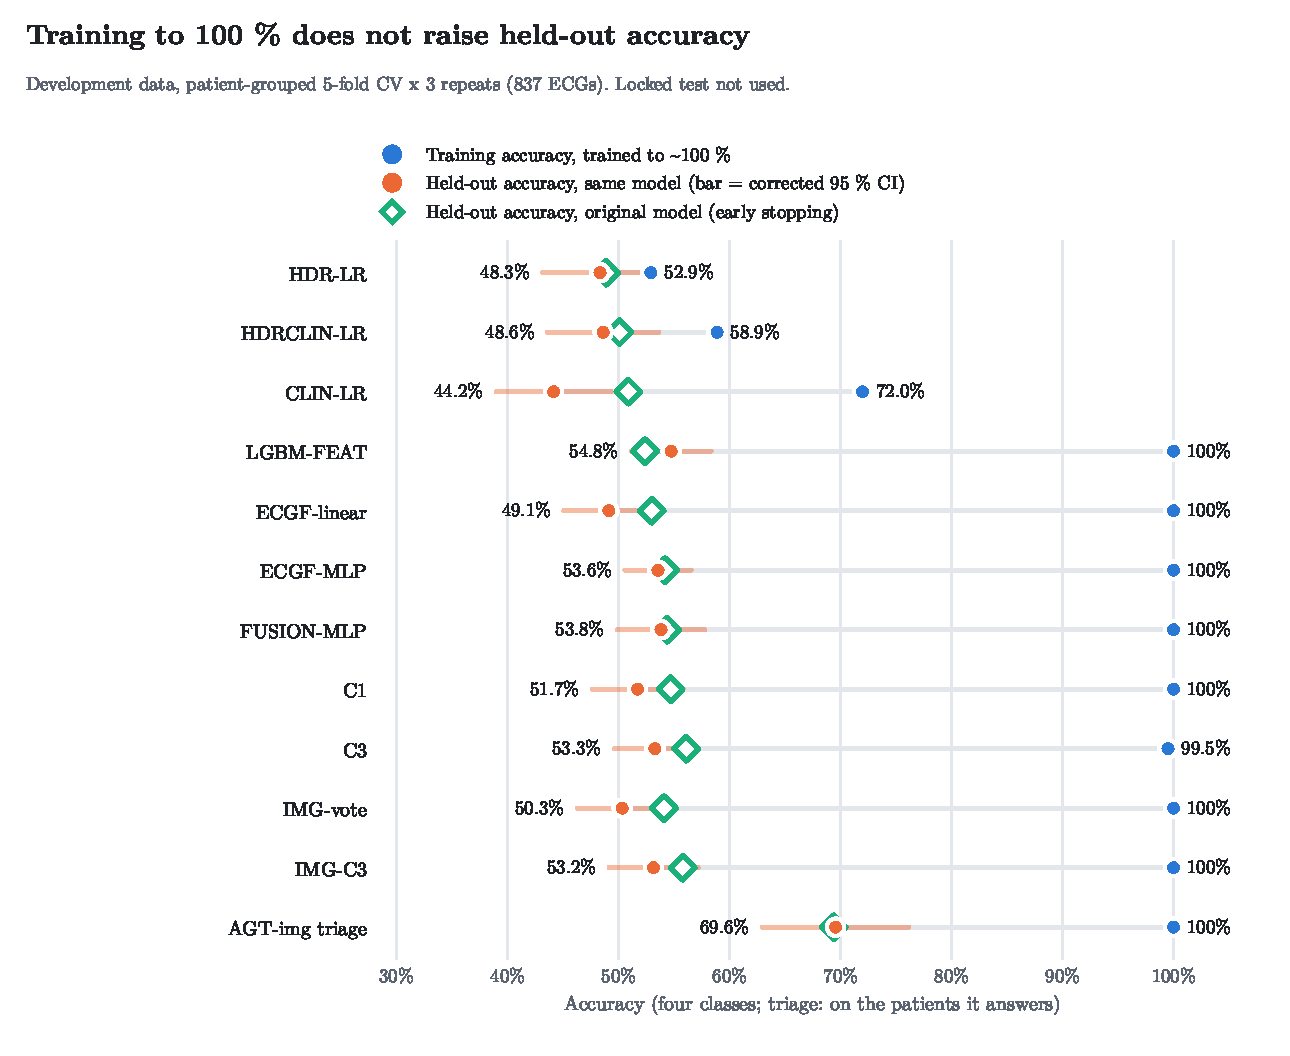
\includegraphics[width=0.97\linewidth,height=0.80\textheight,keepaspectratio]{figures/fig_7_1}
\caption{Development cross-validation: training accuracy after training to (nearly) 100 \% (blue), held-out accuracy of the same model with its corrected 95 \% interval (orange) and held-out accuracy of the original early-stopped model (green).}\label{fig:7.1}
\end{figure}

\section{Image and signal networks on the fixed split}\label{sec:7.3}

Table~\ref{tab:7.3} and Figure~\ref{fig:7.2} show the networks of the original project and Phase 1 on the original fixed split. All seven networks reached at least 0.996 training accuracy, in 12 (ECGFounder fine-tuning) to 57 epochs (MobileNetV3), so none needed the epoch cap. On the 168 validation ECGs, eight of the eleven models lose 0.6--10.7 points: ResNet-18 falls from 0.524 to 0.423, ConvNeXt-Atto from 0.452 to 0.345, the 1-D SE-ResNet from 0.482 to 0.435 and the original default pipeline (header 0.6 + ResNet-18 0.4) from 0.565 to 0.458. Three gain: EfficientNet-B0 (0.351 to 0.417) and MobileNetV3 (0.185 to 0.387) had not yet learnt the task in their original 20--29 epochs, so longer training first helped them, and the ECGFounder fine-tune reached 0.560 against 0.524; on a single 168-ECG split the 95 \% interval is about $\pm$0.075, so this gain is within noise. Every CNN was more accurate on validation at an earlier epoch than at the 100 \% point (ResNet-18 0.482, ECGNet 0.488, EfficientNet-B0 0.512, ConvNeXt-Atto 0.518, 1-D SE-ResNet 0.542, against 0.345--0.435 at the end): the best stopping point lies before 100 \% training accuracy. The header logistic regression again stops at 0.674 training accuracy.

\begin{table}[htbp]
\caption{Image and signal networks on the original fixed split (trained on 669 ECGs, measured on 168 validation ECGs; the locked test is not loaded). TRAIN100: no early stopping, augmentation, weight decay, label smoothing or EMA, trained until training accuracy $\ge$ 99.5 \%. Original training accuracy was measured during the epoch with augmentation and dropout active.}\label{tab:7.3}
\small
\begin{tabular}{>{\raggedright\arraybackslash\hspace{0pt}}p{\dimexpr 0.270\linewidth-2\tabcolsep\relax}>{\raggedright\arraybackslash\hspace{0pt}}p{\dimexpr 0.100\linewidth-2\tabcolsep\relax}>{\raggedright\arraybackslash\hspace{0pt}}p{\dimexpr 0.150\linewidth-2\tabcolsep\relax}>{\raggedright\arraybackslash\hspace{0pt}}p{\dimexpr 0.160\linewidth-2\tabcolsep\relax}>{\raggedright\arraybackslash\hspace{0pt}}p{\dimexpr 0.190\linewidth-2\tabcolsep\relax}>{\raggedright\arraybackslash\hspace{0pt}}p{\dimexpr 0.130\linewidth-2\tabcolsep\relax}}
\toprule
\textbf{Model} & \textbf{Epochs} & \textbf{Training (TRAIN100)} & \textbf{Validation (TRAIN100)} & \textbf{Original: training / validation} & \textbf{Change (points)} \\
\midrule
ResNet-18 & 24 & 0.997 & 0.423 & 0.515 / 0.524 & -10.1 \\
ECGNet & 21 & 0.999 & 0.435 & 0.523 / 0.476 & -4.1 \\
EfficientNet-B0 & 37 & 1.000 & 0.417 & 0.447 / 0.351 & +6.6 \\
ECGFounder fine-tuned (stages 5--6) & 12 & 0.996 & 0.560 & -- / 0.524 & +3.6 \\
HOG + RBF-SVM & -- & 1.000 & 0.423 & -- / 0.458 & -3.5 \\
XGBoost (waveform features) & -- & 1.000 & 0.494 & -- / 0.500 & -0.6 \\
Logistic regression (header) & -- & 0.674 & 0.405 & -- / 0.500 & -9.5 \\
Header 0.6 + ResNet-18 0.4 & -- & 0.972 & 0.458 & -- / 0.565 & -10.7 \\
\bottomrule
\end{tabular}
\end{table}


\begin{figure}[htbp]
\centering
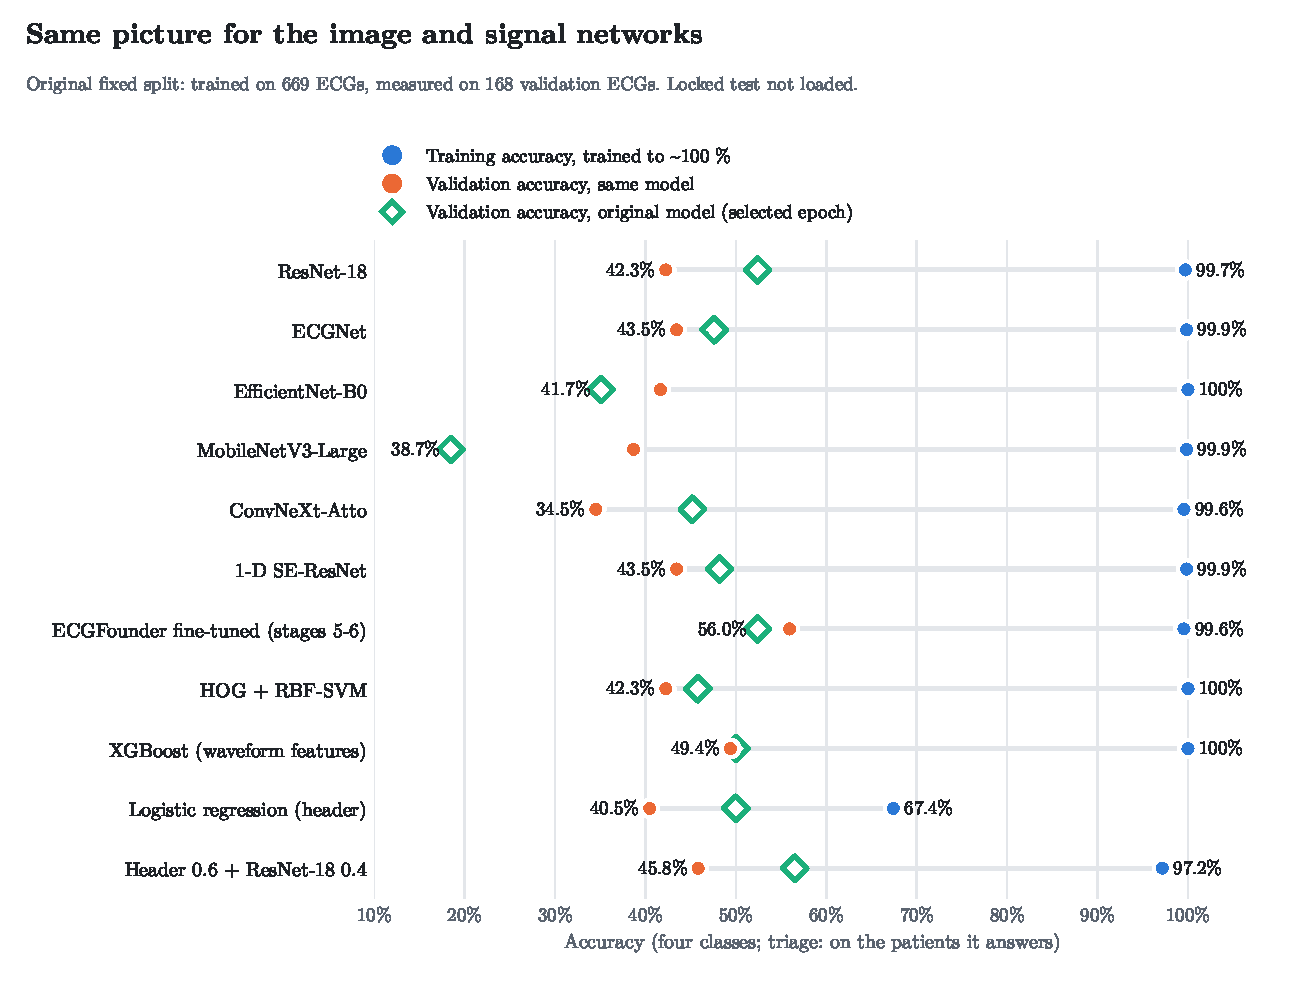
\includegraphics[width=0.97\linewidth,height=0.80\textheight,keepaspectratio]{figures/fig_7_2}
\caption{Original fixed split: training accuracy after training to $\ge$ 99.5 \% (blue), validation accuracy of the same network (orange) and validation accuracy of the original network at its selected epoch (green).}\label{fig:7.2}
\end{figure}

\section{Variants of every phase}\label{sec:7.4}

Table~\ref{tab:7.4} repeats the experiment for the variants of Phases 4, 5 and 6B. The flexible variants again reach 1.000 on their training folds, and their held-out accuracy (0.53--0.56) is the same as or below the original in every case except E2 LightGBM (+1.3 points, inside its interval). The image-only ensembles lose most: HIER 3.5, ENH-vote 2.0 and the ULT stack 3.4 points, because each of their members over-fits in a different way and the errors no longer cancel. Combiners whose decision rule is tuned on out-of-fold member outputs (stacking 0.826, ULT-stack 0.794, SUPER-TOP10-ORD 0.783) do not reach 1.000 in training: their rule is fitted to how the members behave on unseen patients, not to the over-confident in-sample outputs.

The best-for-50s recipe (SUPER-TOP10-ORD, Section~\ref{sec:5.2}) could only be rebuilt from the hospital-trained members of its pool, because the EchoNext data stay on the owner's computer. With the original training, these nine members give 0.565 [0.540, 0.590], so the EchoNext members were worth about 2 points of the published 0.587; trained to 100 \%, the same recipe gives 0.539.

\begin{table}[htbp]
\caption{Variants of every phase, trained to (nearly) 100 \% training accuracy in the same development cross-validation. Members without an original stand-alone result show --.}\label{tab:7.4}
\small
\begin{tabular}{>{\raggedright\arraybackslash\hspace{0pt}}p{\dimexpr 0.360\linewidth-2\tabcolsep\relax}>{\raggedright\arraybackslash\hspace{0pt}}p{\dimexpr 0.130\linewidth-2\tabcolsep\relax}>{\raggedright\arraybackslash\hspace{0pt}}p{\dimexpr 0.250\linewidth-2\tabcolsep\relax}>{\raggedright\arraybackslash\hspace{0pt}}p{\dimexpr 0.130\linewidth-2\tabcolsep\relax}>{\raggedright\arraybackslash\hspace{0pt}}p{\dimexpr 0.130\linewidth-2\tabcolsep\relax}}
\toprule
\textbf{Model} & \textbf{Training (TRAIN100)} & \textbf{Held-out (TRAIN100) [95 \% CI]} & \textbf{Held-out (original)} & \textbf{Change (points)} \\
\midrule
\multicolumn{5}{>{\raggedright\arraybackslash\hspace{0pt}}p{\dimexpr\linewidth-2\tabcolsep\relax}}{\textit{Phase 5 variants}} \\
E1 MLP, header + ECGFounder + feature families & 1.000 & 0.542 [0.504, 0.579] & 0.554 & -1.2 \\
E2 LightGBM, features + ECGFounder PCA & 1.000 & 0.557 [0.517, 0.597] & 0.544 & +1.3 \\
E3 weighted average of the C1 members & 0.985 & 0.530 [0.480, 0.581] & 0.547 & -1.7 \\
E3 stacking (logistic meta-learner) & 0.826 & 0.532 [0.487, 0.576] & 0.546 & -1.4 \\
E4 hierarchical MLP & 0.999 & 0.540 [0.517, 0.563] & 0.567 & -2.7 \\
E6 signal-quality gating & 0.988 & 0.542 [0.500, 0.583] & 0.546 & -0.4 \\
E7 mixup MLP & 1.000 & 0.534 [0.499, 0.570] & 0.552 & -1.8 \\
\multicolumn{5}{>{\raggedright\arraybackslash\hspace{0pt}}p{\dimexpr\linewidth-2\tabcolsep\relax}}{\textit{Phase 4}} \\
Multitask MLP (class + EF) & 1.000 & 0.536 [0.496, 0.577] & 0.546 & -1.0 \\
\multicolumn{5}{>{\raggedright\arraybackslash\hspace{0pt}}p{\dimexpr\linewidth-2\tabcolsep\relax}}{\textit{Phase 6B image-only models}} \\
HIER two-stage (ext. grid) & 1.000 & 0.535 [0.488, 0.582] & 0.570 & -3.5 \\
ENH M2 synthetic 10-s ECG $\rightarrow$ ECGFounder & 1.000 & 0.489 [0.439, 0.539] & 0.528 & -3.9 \\
ENH M3 median-beat shape & 1.000 & 0.412 [0.358, 0.466] & 0.467 & -5.5 \\
ENH M4 MiniRocket & 1.000 & 0.469 [0.423, 0.515] & 0.504 & -3.5 \\
ENH M5 logistic regression & 1.000 & 0.501 [0.450, 0.553] & 0.543 & -4.2 \\
ENH M6 EF ridge $\rightarrow$ bands & 0.557 & 0.477 [0.458, 0.496] & 0.534 & -5.7 \\
ENH-vote & 1.000 & 0.549 [0.513, 0.585] & 0.569 & -2.0 \\
ULT M8 multi-scale ECGFounder LR & 1.000 & 0.496 [0.459, 0.532] & -- & -- \\
ULT M9 kNN & 1.000 & 0.546 [0.520, 0.571] & -- & -- \\
ULT M10 gradient boosting & 1.000 & 0.540 [0.496, 0.585] & -- & -- \\
ULT M12 zone LR & 0.624 & 0.349 [0.302, 0.396] & -- & -- \\
ULT-stack & 0.794 & 0.537 [0.500, 0.574] & 0.571 & -3.4 \\
\multicolumn{5}{>{\raggedright\arraybackslash\hspace{0pt}}p{\dimexpr\linewidth-2\tabcolsep\relax}}{\textit{Best-for-50s recipe without EchoNext (original column: same recipe on the original members; the published 0.587 also used EchoNext members)}} \\
SUPER-TOP10-ORD, hospital members only & 0.783 & 0.539 [0.509, 0.570] & 0.565 & -2.6 \\
\bottomrule
\end{tabular}
\end{table}


The EF regressors show the same pattern in Table~\ref{tab:7.5}: the MLP reproduces the training EF almost exactly ($r$ = 0.993, mean error 2.7 points) but its held-out correlation falls from 0.653 to 0.624, and the unshrunk ridge + LightGBM regressor drops to $r$ = 0.476.

\begin{table}[htbp]
\caption{EF regression (Phase 4) trained without early stopping: correlation with echo EF on the training rows and held out, and mean absolute error in EF points.}\label{tab:7.5}
\small
\begin{tabular}{>{\raggedright\arraybackslash\hspace{0pt}}p{\dimexpr 0.360\linewidth-2\tabcolsep\relax}>{\raggedright\arraybackslash\hspace{0pt}}p{\dimexpr 0.140\linewidth-2\tabcolsep\relax}>{\raggedright\arraybackslash\hspace{0pt}}p{\dimexpr 0.140\linewidth-2\tabcolsep\relax}>{\raggedright\arraybackslash\hspace{0pt}}p{\dimexpr 0.200\linewidth-2\tabcolsep\relax}>{\raggedright\arraybackslash\hspace{0pt}}p{\dimexpr 0.160\linewidth-2\tabcolsep\relax}}
\toprule
\textbf{Regressor} & \textbf{Training $r$} & \textbf{Held-out $r$} & \textbf{MAE training / held-out} & \textbf{Original held-out $r$} \\
\midrule
EF regression MLP, header + ECGFounder & 0.993 & 0.624 & 2.7 / 11.0 & 0.653 \\
EF ridge + LightGBM (triage regressor) & 1.000 & 0.476 & 0.0 / 13.8 & -- \\
\bottomrule
\end{tabular}
\end{table}


\section{Label-quality studies}\label{sec:7.5}

Table~\ref{tab:7.6} repeats the label-quality studies of Table~\ref{tab:4.7} with the C3 recipe trained to (nearly) 100 \%. Training on cleaner labels still pays off on the clean subsets (0.67--0.69 on the clear-cut and noise-free ECGs), but none of the studies gains from the longer training: CLEAR, MMCLEAN and NFS stay within one point of their originals (0.670 against 0.668, 0.669 against 0.672, 0.694 against 0.702), and HC30, NF and VER lose 1.0--2.8 points. Cleaner labels raise accuracy; more training does not.

\begin{table}[htbp]
\caption{Label-quality studies (report Table 4.7) with the C3 recipe trained to (nearly) 100 \% training accuracy, scored on the same subsets as the original.}\label{tab:7.6}
\small
\begin{tabular}{>{\raggedright\arraybackslash\hspace{0pt}}p{\dimexpr 0.220\linewidth-2\tabcolsep\relax}>{\raggedright\arraybackslash\hspace{0pt}}p{\dimexpr 0.160\linewidth-2\tabcolsep\relax}>{\raggedright\arraybackslash\hspace{0pt}}p{\dimexpr 0.150\linewidth-2\tabcolsep\relax}>{\raggedright\arraybackslash\hspace{0pt}}p{\dimexpr 0.160\linewidth-2\tabcolsep\relax}>{\raggedright\arraybackslash\hspace{0pt}}p{\dimexpr 0.160\linewidth-2\tabcolsep\relax}>{\raggedright\arraybackslash\hspace{0pt}}p{\dimexpr 0.150\linewidth-2\tabcolsep\relax}}
\toprule
\textbf{Study} & \textbf{Scored on} & \textbf{Training accuracy} & \textbf{Accuracy} & \textbf{Original} & \textbf{Change (points)} \\
\midrule
VER: 15 labels corrected to a high-confidence echo & all 837 (original labels) & 0.986 & 0.537 & 0.565 & -2.8 \\
HC30: train on reliable links only & 395 reliable links & 1.000 & 0.583 & 0.594 & -1.1 \\
CLEAR: train without border ECGs & 582 clear-cut ECGs & 0.993 & 0.670 & 0.668 & +0.2 \\
MMCLEAN: drop suspect Mild/Moderate labels & 620 kept ECGs & 0.978 & 0.669 & 0.672 & -0.3 \\
NF: noise-free training (all classes) & 264 clean, clear-cut ECGs & 1.000 & 0.673 & 0.683 & -1.0 \\
NFS: noise-free training, Severe kept & 264 clean, clear-cut ECGs & 0.985 & 0.694 & 0.702 & -0.8 \\
\bottomrule
\end{tabular}
\end{table}


\section{Models that were not retrained}\label{sec:7.6}

Table~\ref{tab:7.7} lists what was left out and why. The best-in-the-70s result (0.747 on the locked test) stays with the original frozen model: the locked test was scored once with the owner's authorisation, and scoring it again would remove its value as an unseen test.

\begin{table}[htbp]
\caption{Models not retrained in TRAIN100, and why.}\label{tab:7.7}
\small
\begin{tabular}{>{\raggedright\arraybackslash\hspace{0pt}}p{\dimexpr 0.420\linewidth-2\tabcolsep\relax}>{\raggedright\arraybackslash\hspace{0pt}}p{\dimexpr 0.580\linewidth-2\tabcolsep\relax}}
\toprule
\textbf{Model} & \textbf{Reason} \\
\midrule
SUPER / STAGED-4 / ULT2 ensembles with EchoNext members, EchoNext-only models (EN-cls, EN-all), EchoNext-pre-trained pixel CNNs (ZS, FT-EN, ConvNeXt E2--E6, IMG70) & EchoNext data are under a PhysioNet credentialed data-use agreement and stay on the owner's computer; the best-for-50s recipe was rebuilt from its hospital-only members instead (Table~\ref{tab:7.4}) \\
Locked-test result (best in the 70s, 0.747) & the 210 locked ECGs were scored once with the owner's authorisation; scoring them again would remove their value as an unseen test \\
LSTM family (L0--L5) and LSTM fusions & withdrawn at the owner's request: the LSTMs did not raise accuracy in Phase 6 (Tables~\ref{tab:4.5}--\ref{tab:4.6}); one CNN-LSTM test fold reached 0.997 training and 0.446 held-out accuracy \\
EfficientNet-B2 and ConvNeXt-Tiny (IMG70 architectures) & left out at the owner's request (7--16 CPU-minutes per epoch here); their originals were EchoNext-pre-trained \\
E7 augmentation, MMCLEAN grid configurations, HC30F, selective prediction & inputs not on this machine, not in Table~\ref{tab:4.7}, or the same idea as the triage model \\
\bottomrule
\end{tabular}
\end{table}


\section{Why training to 100 \% does not help, and where to stop}\label{sec:7.7}

Figure~\ref{fig:7.3} follows the ECGFounder MLP head epoch by epoch for 150 epochs on the five folds of repeat 0. Training accuracy rises to 1.000, while held-out accuracy stops improving after about 12 epochs and then stays flat or falls. With the project's regularised head, the early-stopping point (epoch 12 on average) gives 0.823 training and 0.519 held-out accuracy; after 150 epochs the same head is at 1.000 and 0.520. Without dropout or weight decay, held-out accuracy falls from 0.545 at the stopping point to 0.529 at epoch 150.

The reason is the size of the problem. Each training fold holds about 670 ECGs, while the networks have between 66,000 (MLP head) and 30.8 million (ECGFounder) parameters, and many labels are uncertain: the label studies of Section~\ref{sec:4.4} found 217 suspect Mild/Moderate labels and links that are more than 30 days or a name match away from the echo. Once a model has learnt the patterns that generalise, the only way to raise training accuracy further is to memorise the individual training ECGs, including their noise and label errors. That memorised detail does not exist in new patients, so held-out accuracy cannot rise and often falls.

The best stopping point is therefore not 100 \% training accuracy but the epoch at which accuracy on data the model has not seen stops improving. In this project that is the inner-validation early-stopping point used in all original runs, where training accuracy is about 0.60--0.85. The gap between training and held-out accuracy is the measure of over-fitting, and the held-out accuracy is the number to report.

\begin{figure}[htbp]
\centering
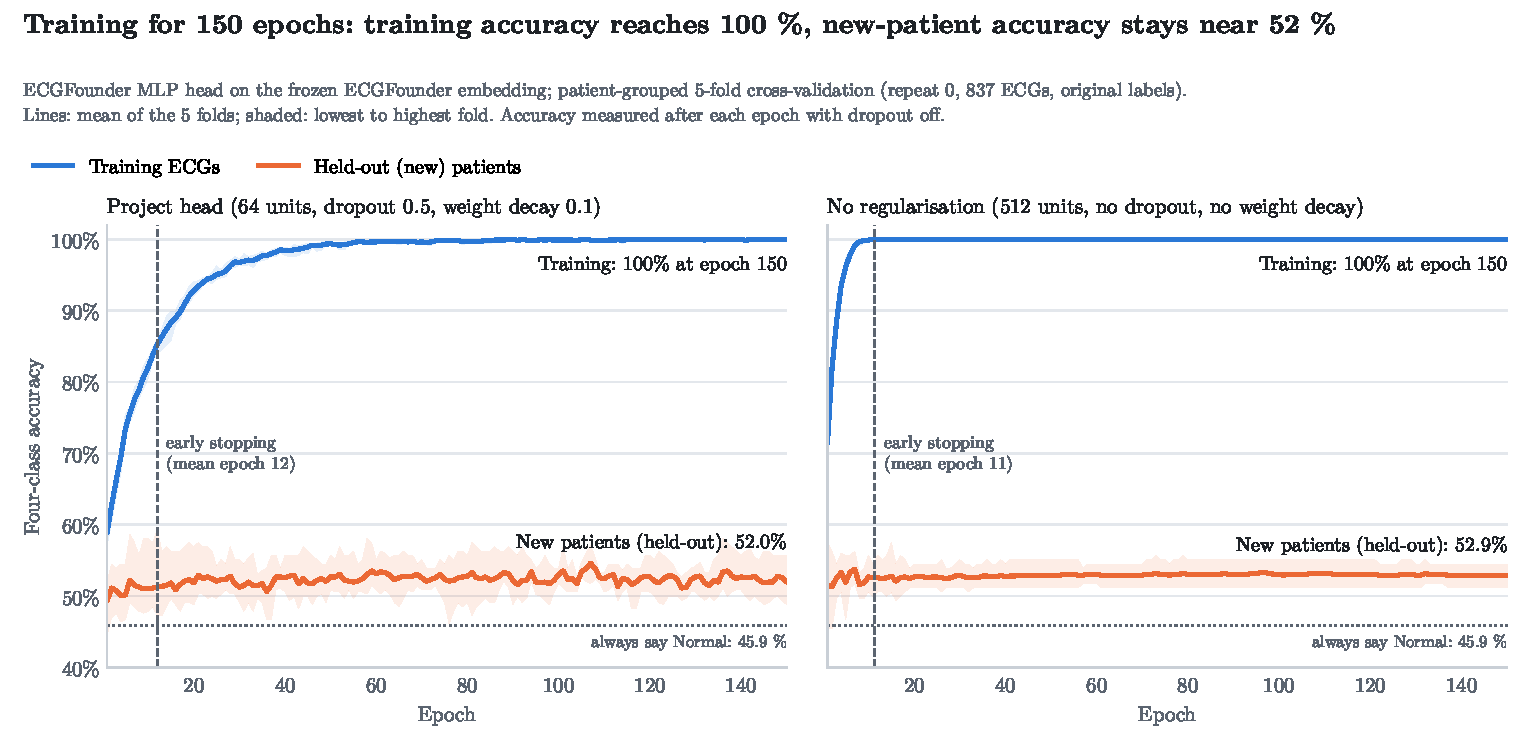
\includegraphics[width=0.97\linewidth,height=0.80\textheight,keepaspectratio]{figures/fig_7_3}
\caption{ECGFounder MLP head trained for 150 epochs without early stopping (mean of the five folds of repeat 0): training accuracy reaches 1.000 while held-out accuracy stays at about 0.52. Left: the project head; right: the same head without dropout or weight decay. The dashed line marks the early-stopping epoch.}\label{fig:7.3}
\end{figure}
